\documentclass[11pt, a4paper]{article}
\usepackage{config}


%%%%%%%%
% Title
%%%%%%%%
% \begin{titlepage}
  \begin{center}
    \vspace*{1cm}

    \Huge
    \textbf{Template document}

    \vspace{0.5cm}
    \LARGE

    TITLE PAGE

    \vspace{1.5cm}

    \texttt{Yuya HAGA}
    \texttt{00-00-0000}

    \vspace{0.8cm}
    %\vspace{3cm}
    %\vfill
    %\includegraphics[width=0.8\textwidth]{images/imatge_portada.png}
    % \missingfigure{Add a picture for the front page.}

    \vfill

    \Large
    \missingfigure{Add a picture of a logo.}

  \end{center}
\end{titlepage}


%%%%%%%%
%%%%%%%%


%add author information on left side on top of the page
\author{Yuya Haga}
\title{Advanced Spectral Imaging: Homework 1}
\date{\today}


% Header and footer
\pagestyle{fancy}
\fancyhf{}
\rhead{Homework 1}
\chead{
\includegraphics[width=1.5cm]{images/UEF_logo.png}}
\lhead{Advanced Spectral Imaging}
\rfoot{\thepage}

% \section{Figures}
Single figure:
\begin{figure}[H] %
  \centering
  \includegraphics[width=0.5\textwidth]{images/giraffe.jpg}
  \caption[]{Caption}
  \label{fig:label}
\end{figure}

Subfigures:
\begin{figure}[H] %
  \centering
  \subfloat[SubcaptionA]{\includegraphics[width=0.45\textwidth]{images/giraffe.jpg}}
  \hspace{0.1cm}
  \subfloat[SubcaptioB]{\includegraphics[width=0.45\textwidth]{images/giraffe.jpg}}
  \caption[]{Caption}
  \label{fig:label}
\end{figure}

\section{Tables}
You can use this link for tables: \url{https://www.tablesgenerator.com/}

Table:
\begin{table}[H]
  \centering
  %\resizebox{\textwidth}{!} %%%% Activate if it's a long table
  {
    \begin{tabular}{|l|c|r|}
      \hline
      \textbf{Left} & \textbf{Center} & \textbf{Right} \\ \hline \hline
      1 & 2 & 3 \\ \hline
      4 & 5 & 6 \\ \hline
      7 & 8 & 9 \\ \hline

  \end{tabular}}
  \caption{Caption}
  \label{tab:label}
\end{table}

Long table:
\begin{table}[H]
  \centering
  \resizebox{\textwidth}{!}{
    \begin{tabular}{|r|r|r|r|r|r|}
      \hline
      \textbf{TitleVeryVeryLong1} & \textbf{Title2} &
      \textbf{TitleVeryVeryLong3} & \textbf{Title4} &
      \textbf{TitleVeryVeryLong5} & \textbf{Title6} \\ \hline \hline
      1 &2& 3 & 4 & 5  & 6 \\ \hline
      1 &2& 3 & 4 & 5  & 6 \\ \hline

  \end{tabular}}
  \caption{Caption}
  \label{tab:label}
\end{table}

\clearpage
\section{Pseudocode}

Example of simple algorithm:
\begin{algorithm}[H]
  \caption{AlgorithmDescription}
  \label{alg:label}
  \textbf{Input:} Define the input\\
  \textbf{Output:} Define the output

  \begin{algorithmic}[1]
    \STATE Do an operation
    \STATE Do another operation
    \STATE Wait some miliseconds
    \IF{Condition}
    \STATE Do corresponding action
    \ENDIF
    \STATE Do something else
    \STATE \textbf{return} $-1$
  \end{algorithmic}
\end{algorithm}

Example of algorithm with functions predefined:

\begin{algorithm}[H]
  \caption{AlgorithmDescription}
  \label{alg:label}
  \textbf{Input:} Graf $G = (V, E)$ no dirigit i connex, Vector
  d'enters \emph{NND}\\
  \textbf{Output:} \emph{-1} si NND és un conjunt dominador, $i \in
  [0, N)$ altrament
  \begin{algorithmic}[1]
    %For
    \FOR{each $i \in [0, N)$}
    \STATE Do something
    \ENDFOR

    \STATE Explain somehting like "Generakte k+1 neighbors"

    \IF{$NND[i] < \left\lceil
    \displaystyle\frac{G.get\_nb\_veins(i)}{2} \right\rceil$}
    \STATE \textbf{return} $i$
    \ENDIF

    \WHILE{D is not a PIDS}
    \STATE $v* \leftarrow arg max_{\forall v \not\in S } \{funcioGreedy(v)\}$
    \STATE $D \leftarrow  D  \cup  \{v*\}$
    \STATE $updateData(v)$
    \ENDWHILE
    \STATE \textbf{return} $-1$
  \end{algorithmic}
\end{algorithm}

\section{Code fragments}
\begin{lstlisting}[language=Python, caption={CaptionPythonCode}, label={code:label}]
## Insert here the code as it
## Change the language from the headder to adapt the colors

def __main__():
    print("Hello World!")
\end{lstlisting}

% \clearpage
%--------------------to clear---------------------------



\begin{document}
\fancypagestyle{plain}{} % <-- new
\maketitle

\section{Task \#1. Segmentation of green materials}

Segmentation results of green materials by Nuance camera is shown in Figure \ref{fig:green-nuance}.
Codes for this task can be found in Code \ref{code:green-nuance}.

\begin{figure}[H]
    \centering
    \caption{Segmentation results by Nuance camera}
    \label{fig:green-nuance}
    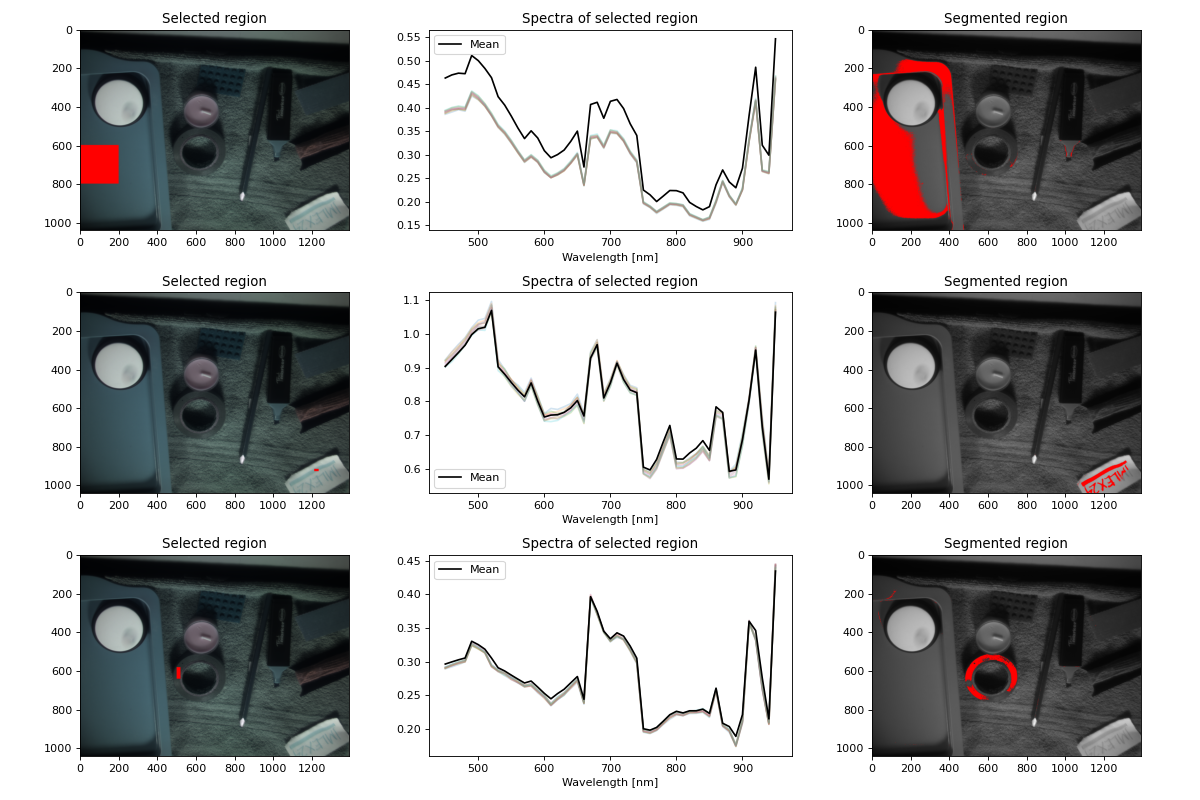
\includegraphics[width=0.75\textwidth]{./fig/task1/nuance.png}
\end{figure}

Segmentation results of green materials by Tuneble light camera is
shown in Figure \ref{fig:green-tunable}.
Codes for this task can be found in Code \ref{code:green-tunable}.

\begin{figure}[H]
  \centering
  \caption{Segmentation results by Tunable light camera}
  \label{fig:green-tunable}
  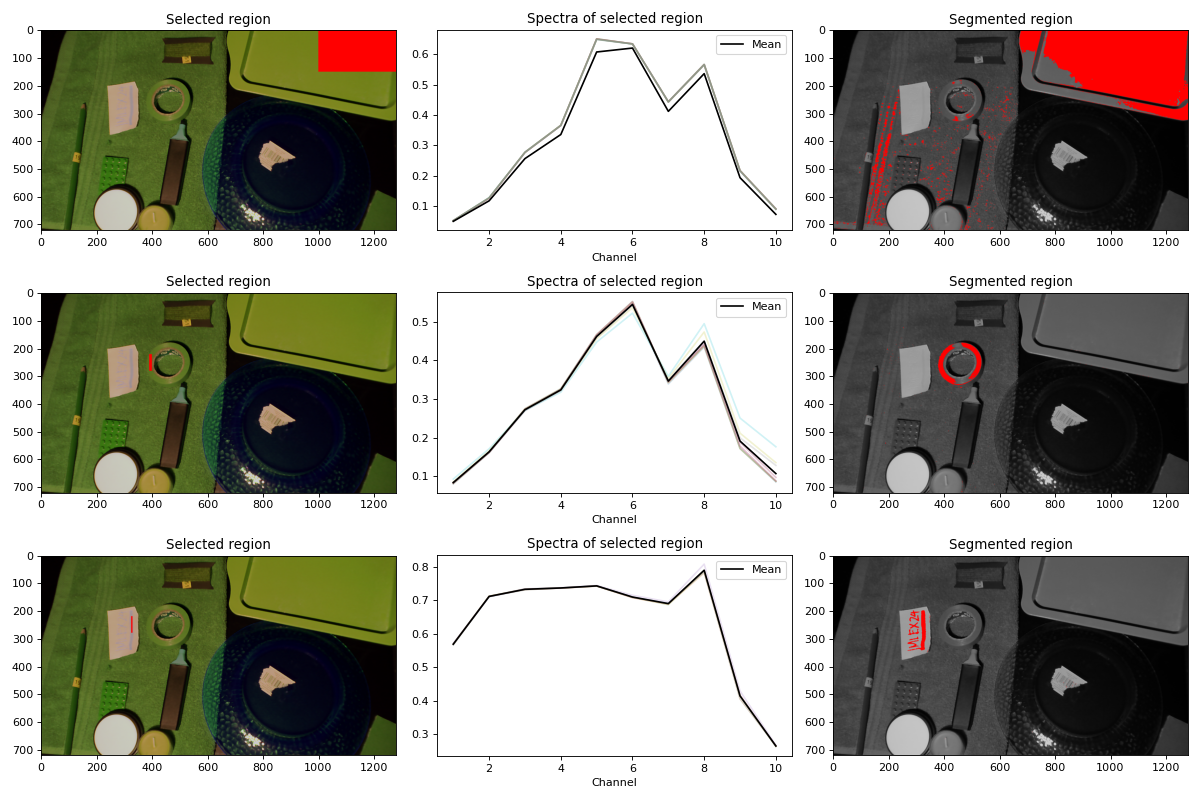
\includegraphics[width=0.75\textwidth]{./fig/task1/tunable.png}
\end{figure}
Segmentation results of green materials by Specim Scanner in visible
wavelengths is shown in Figure \ref{fig:green-specim-vis}.
Codes for this task can be found in Code \ref{code:green-specim-vis}.
\begin{figure}[H]
  \centering
  \caption{Segmentation results by Specim Scanner in visible wavelengths}
  \label{fig:green-specim-vis}
  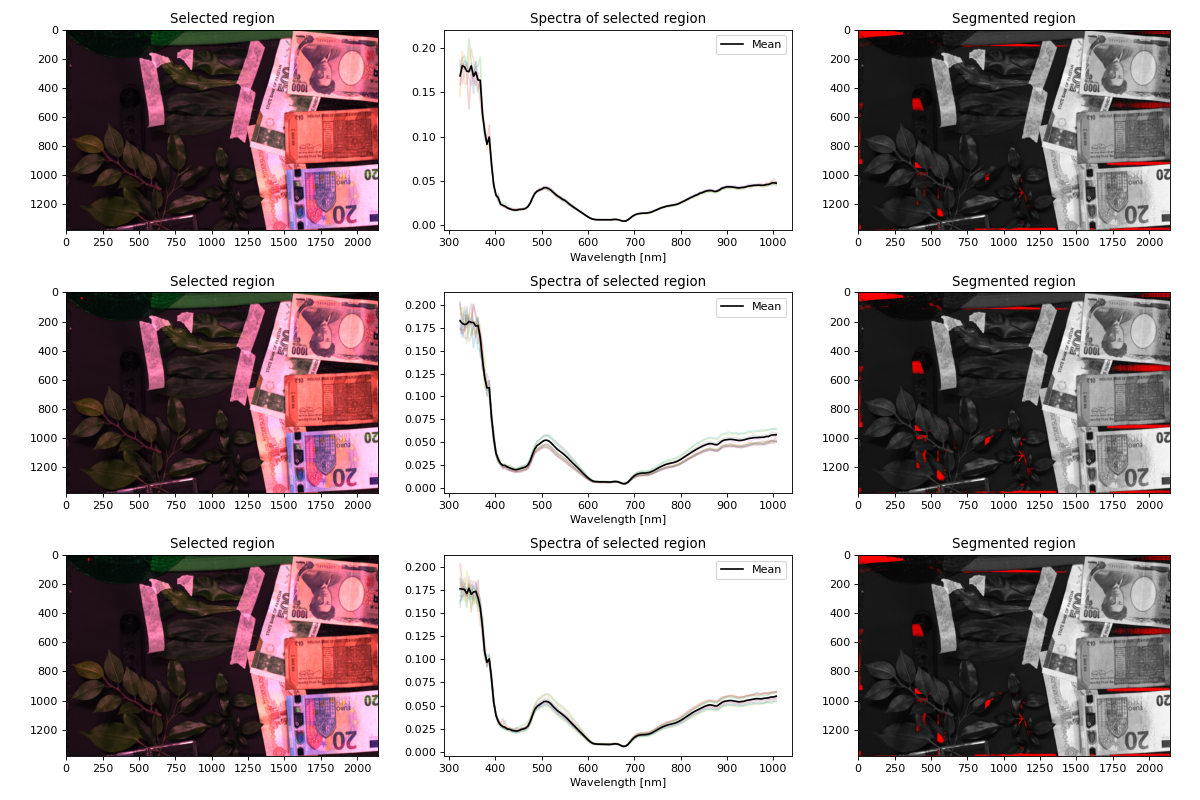
\includegraphics[width=0.75\textwidth]{./fig/task1/specim-scanner-vis.png}
\end{figure}

Segmentation results of green materials by Specim Scanner in infrared
wavelengths is shown in Figure \ref{fig:green-specim-ir}.
Codes for this task can be found in Code \ref{code:green-specim-ir}.
\begin{figure}[H]
  \centering
  \caption{Segmentation results by Specim Scanner in infrared wavelengths}
  \label{fig:green-specim-ir}
  \includegraphics[width=0.75\textwidth]{./fig/task1/specim-scanner-ir.png}
\end{figure}


\section{Task \#2. Plastic green leaves}

Segmentation of leaves by SpecimIQ in visible wavelengths is shown in
Figure \ref{fig:leaves-specim-iq}.
Codes for this task can be found in Code \ref{code:leaves-specim-iq}.

\begin{figure}[H]
  \centering
  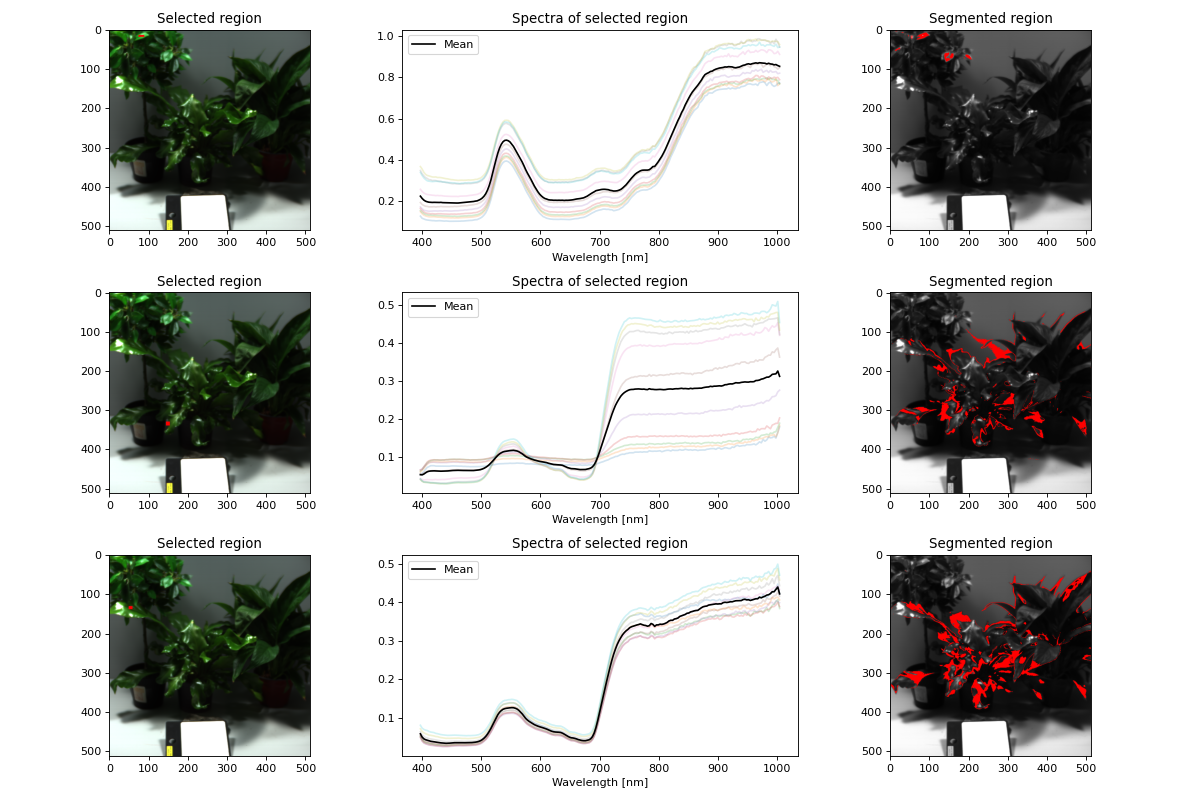
\includegraphics[width=0.8\textwidth]{./fig/task2/specim-iq.png}
  \caption{Segmentation of leaves by Specim Scanner }
  \label{fig:leaves-specim-iq}
\end{figure}
c
Segmentation results of leaves by Specim Scanner in infrared
wavelengths is shown in Figure \ref{fig:leaves-specim-ir}.
Codes for this task can be found in Code \ref{code:leaves-specim-ir}.
\begin{figure}[H]
  \centering
  \caption{Segmentation results by Specim Scanner in infrared wavelengths}
  \label{fig:leaves-specim-ir}
  \includegraphics[width=0.75\textwidth]{./fig/task2/specim-scanner-ir.png}
\end{figure}


\section{Task \#3. powders / medical image}

c
Segmentation of white powders by Specim Scanner in infrared wavelengths is operated in two ways.

First method is to use the selected areas for segmentation. The selected areas and results are shown in Figure \ref{fig:powder-specim-ir-1}. 

The codes for this task can be found in Code \ref{code:powder}.

\begin{figure}[H]
  \centering
  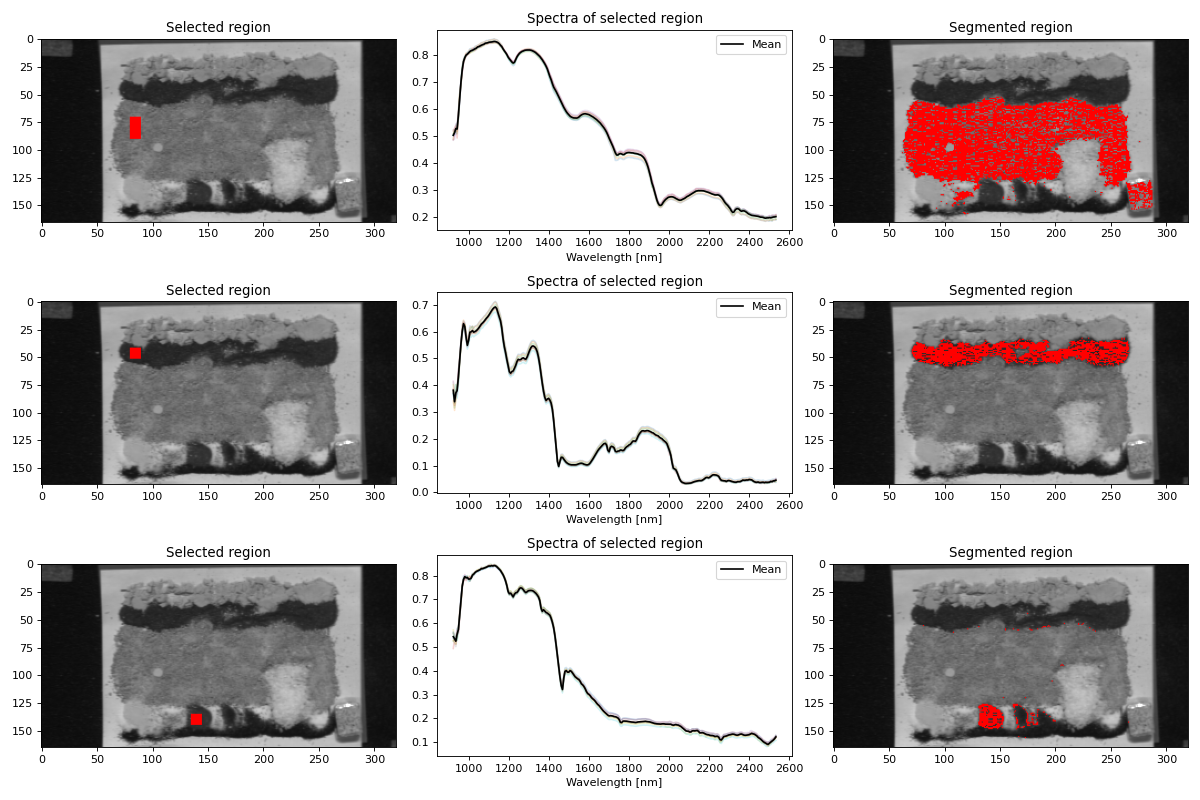
\includegraphics[width=0.8\textwidth]{./fig/task3/powder.png}
  \caption{Selected areas for segmentation by Specim Scanner in infrared wavelengths}
  \label{fig:powder}
\end{figure}

Second method is to use RGB visualization of the spectral image. The segmentation results are shown in Figure \ref{fig:powder-seg}

The codes for this task can be found in Code \ref{code:powder-segment}.

\begin{figure}[H]
  \centering
  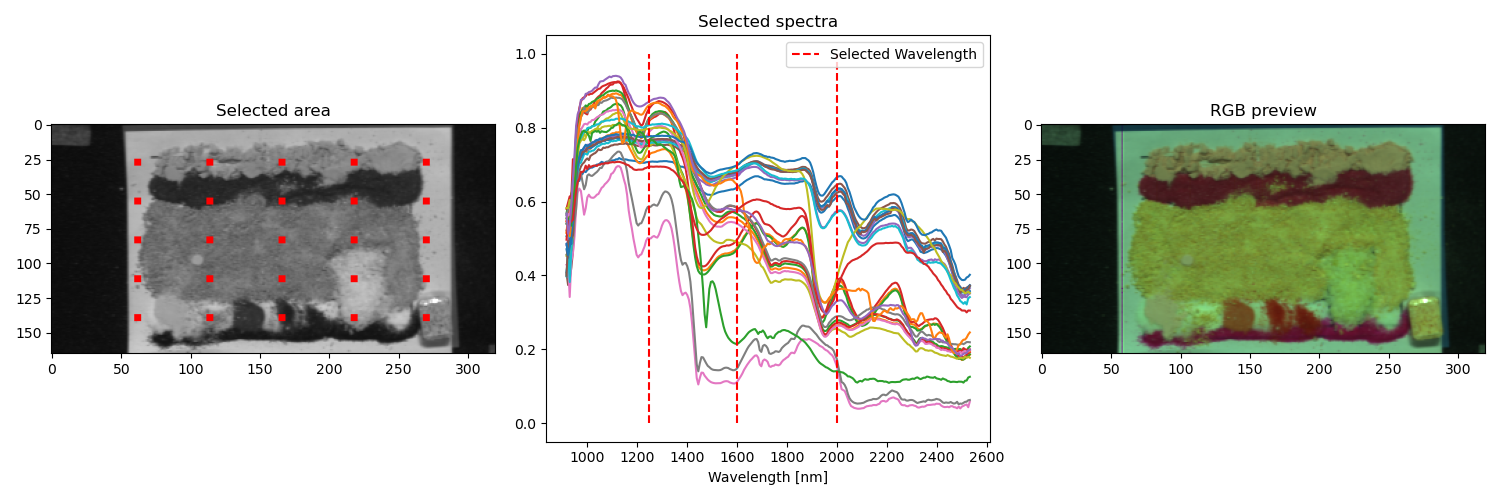
\includegraphics[width=0.8\textwidth]{./fig/task3/powder-segment.png}
  \caption{Segmentation results by Specim Scanner in infrared wavelengths}
  \label{fig:powder-seg}
\end{figure}


\section{Codes}
\begin{lstlisting}[language=python, caption=Segmentation of green materials by Nuance camera, label={code:green-nuance}]
import matplotlib.pyplot as plt
import numpy as np

from asi import path_config
from asi.draw import reconstruct_rgb
from asi.io.load_nuance import load_nuance_image
from segmentation import plot_segmentation_results

# Load spectral image and apply white correction
session2 = path_config.measurements / "session2"
nuance = session2 / "Nuance"
root = nuance / "greenmaterials"

# load spectral image
spectral_image, wavelengths = load_nuance_image(root)
spectral_image = spectral_image.astype(np.float64)

white_pos = (slice(320, 400), slice(100, 200))

# White correction with selected area
white_sq = spectral_image[white_pos]

# replace nonzero elements with minimum value
nonzero_elements = white_sq[white_sq != 0]
min_elm = nonzero_elements.min()
white_sq = white_sq.clip(min_elm, None)

# apply white correction
whiteref = white_sq.mean(axis=(0, 1))
spectral_image /= whiteref

rgb_view = reconstruct_rgb(spectral_image, wavelengths)


fig, axes = plt.subplots(3, 3, tight_layout=True, figsize=(15, 10), dpi=80)

select_pos = (slice(600, 800), slice(0, 200))
plot_segmentation_results(
    axes[0],
    spectral_image,
    wavelengths,
    select_pos,
    rgb_view,
    threshold=0.11,
)

select_pos = (slice(915, 927), slice(1212, 1235))
plot_segmentation_results(
    axes[1],
    spectral_image,
    wavelengths,
    select_pos,
    rgb_view,
    threshold=0.2,
)
select_pos = (slice(580, 640), slice(500, 520))
plot_segmentation_results(
    axes[2],
    spectral_image,
    wavelengths,
    select_pos,
    rgb_view,
    threshold=0.080,
)

fig.show()
fig.savefig("./fig/task1/nuance.png")

\end{lstlisting}
\begin{lstlisting}[language=python, caption=Segmentation of green materials by Tunable light camera, label={code:green-tunable}]
import matplotlib.pyplot as plt
import numpy as np

from asi import path_config
from asi.io.load_tunable import load_tunable_image
from segmentation import plot_segmentation_results

# Configurations
WHITE_POS = (slice(600, 700), slice(230, 300))
# LOAD IMAGE
session1 = path_config.measurements / "session2"
tunable_root = session1 / "Tunable" / "green materials"

spectral_image, channels = load_tunable_image(
    tunable_root,
    name="colorchecker",
    white_pos=WHITE_POS,
)
spectral_image = spectral_image.astype(np.float64)

# Apply white correction
white_sq = spectral_image[WHITE_POS]
whiteref = white_sq.mean(axis=(0, 1))
white_corrected = spectral_image / whiteref
spectral_image /= spectral_image.max()


# Make RGB view
SELECT_CHANNELS = [7, 5, 1]
# Make RGB view
rgb_view = spectral_image[..., SELECT_CHANNELS]
# Postprocess for preview
rgb_view /= rgb_view.max()
rgb_view *= 0.8
rgb_view = rgb_view.clip(0, 1)

wavelengths = channels

fig, axes = plt.subplots(3, 3, tight_layout=True, figsize=(15, 10), dpi=80)


select_pos = (slice(0, 150), slice(1000, None))
plot_segmentation_results(
    axes[0],
    spectral_image,
    wavelengths,
    select_pos,
    rgb_view,
    threshold=0.1,
)

select_pos = (slice(220, 280), slice(390, 400))
plot_segmentation_results(
    axes[1],
    spectral_image,
    wavelengths,
    select_pos,
    rgb_view,
    threshold=0.05,
)

select_pos = (slice(220, 280), slice(325, 330))
plot_segmentation_results(
    axes[2],
    spectral_image,
    wavelengths,
    select_pos,
    rgb_view,
    threshold=0.11,
)

fig.show()
fig.savefig("./fig/task1/tunable.png")
\end{lstlisting}
\begin{lstlisting}[language=python, caption=Segmentation of green materials by Specim Scnaner in visible wavelengths, label={code:green-specim-vis}]
import matplotlib.pyplot as plt
import numpy as np

from asi import path_config
from asi.draw import reconstruct_rgb_envi
from asi.preprocess import load_white_corrected
from asi.utils import get_wavelengths
from segmentation import plot_segmentation_results

# Load spectral image and apply white correction
session2 = path_config.measurements / "session2"
specim_scanner = session2 / "Specim scanner" / "GreenSamplesVisible" / "capture"

name = "solutions_scan_0145"
image_path = specim_scanner / name
darkref_path = specim_scanner / f"DARKREF_{name}"
whiteref_path = specim_scanner / f"WHITEREF_{name}"

spectral_image, envi_header = load_white_corrected(
    image_path,
    whiteref_path,
    darkref_path,
)
spectral_image = spectral_image.astype(np.float16)

rgb_view = reconstruct_rgb_envi(spectral_image, envi_header)
rgb_view *= 3
rgb_view = rgb_view.clip(0, 1)
wavelengths = get_wavelengths(envi_header)


fig, axes = plt.subplots(3, 3, tight_layout=True, figsize=(15, 10), dpi=80)


select_pos = (slice(1245, 1260), slice(1750, 1770))
plot_segmentation_results(
    axes[0],
    spectral_image,
    wavelengths,
    select_pos,
    rgb_view,
    threshold=0.3,
)
select_pos = (slice(200, 240), slice(1600, 1700))
plot_segmentation_results(
    axes[1],
    spectral_image,
    wavelengths,
    select_pos,
    rgb_view,
    threshold=0.3,
)
select_pos = (slice(200, 400), slice(0, 250))
plot_segmentation_results(
    axes[2],
    spectral_image,
    wavelengths,
    select_pos,
    rgb_view,
)

fig.show()
fig.savefig("./fig/task1/specium-scanner-vis.png")
\end{lstlisting}
\begin{lstlisting}[language=python, caption=Segmentation of green materials by Specim Scnaner in infrared wavelengths, label={code:green-specim-ir}]

import matplotlib.pyplot as plt
import numpy as np

from asi import path_config
from asi.draw import reconstruct_gray_view
from asi.preprocess import load_white_corrected
from asi.utils import get_wavelengths
from segmentation import plot_segmentation_results

# Load spectral image and apply white correction
session2 = path_config.measurements / "session2"
specim_scanner = session2 / "Specim scanner" / "GreenSamplesIR" / "capture"

name = "IR_scan_0463"
image_path = specim_scanner / name
darkref_path = specim_scanner / f"DARKREF_{name}"
whiteref_path = specim_scanner / f"WHITEREF_{name}"

spectral_image, envi_header = load_white_corrected(
    image_path,
    whiteref_path,
    darkref_path,
)
spectral_image = spectral_image.astype(np.float16)

rgb_view = reconstruct_gray_view(spectral_image)
rgb_view *= 1.5
rgb_view = rgb_view.clip(0, 1)
wavelengths = get_wavelengths(envi_header)


fig, axes = plt.subplots(3, 3, tight_layout=True, figsize=(15, 10), dpi=80)


select_pos = (slice(155, 158), slice(261, 264))
plot_segmentation_results(
    axes[0],
    spectral_image,
    wavelengths,
    select_pos,
    rgb_view,
    threshold=0.13,
)
select_pos = (slice(29, 35), slice(238, 245))
plot_segmentation_results(
    axes[1],
    spectral_image,
    wavelengths,
    select_pos,
    rgb_view,
    threshold=0.15,
)
select_pos = (slice(29, 55), slice(0, 30))
plot_segmentation_results(
    axes[2],
    spectral_image,
    wavelengths,
    select_pos,
    rgb_view,
    threshold=0.15,
)

fig.show()
fig.savefig("./fig/task1/specium-scanner-ir.png")
\end{lstlisting}


% \renewcommand\refname{}
\bibliographystyle{plain} % We choose the "plain" reference style
% \bibliographystyle{apalike}
\bibliography{references} % Entries are in the referencies.bib file
%\nocite{*}
% Add all references, even though they are not cited

\end{document}
